\chapter{Documentazione driver per SCO Board}
\label{appendiceA}
\thispagestyle{empty}

\textit{Quest'appendice contiene una breve descrizione dei driver sviluppati per interfacciare la SCO Board con la scheda di prototipazione NI sbRIO-9636}

\section*{VI sviluppati} %% TODO Pensare a un titolo piu bello
Per consentire la comunicazione tra la scheda di conversione \textit{SCO Board} e la \textit{NI sbRIO-9636} è stato necessario lo sviluppo di un apposito driver. Si è scelto di rendere disponibile una versione completa dei driver per consentire il riutilizzo della scheda di conversione per lavori futuri. 
Per la distribuzione si è deciso di fornire un archivio \textit{.zip}, scaricabile da \textit{SourceForge} \cite{sourceforge}, contenente i VI necessari.

I VI che fanno parte del set di driver sviluppato sono:
\begin{itemize}
	\item \textit{Output enable-disable}: Abilita/disabilita i pin digitali di uscita
	\item \textit{Clock enable-disable}: Abilita/disabilita i pin digitali di uscita dedicati ai segnali di clock ADC/DAC
	\item \textit{Clock generator}: Genera il segnale di clock sincrono per DAC ed ADC
	\item \textit{Single point acquisition}: Acquisisce un campione dei dati in ingresso
	\item \textit{Single point generation}: genera un campione di dati sulle uscite
\end{itemize}

Di seguito verrà descritta in dettaglio la struttura di ciascun VI e come utilizzarli all'interno di un software LabVIEW.
Per la descrizione di ingressi ed uscite si è scelto di avvalersi della convenzione di LabVIEW, evidenziando in grassetto gli ingressi necessari all'esecuzione del VI.

\subsection*{Output enable-disable}

\begin{figure}[H]
	\begin{center}
		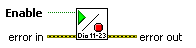
\includegraphics[scale=1]{appendiceA/enable_output}
		\caption{Struttura VI Output enable-disable}
	\end{center}
\end{figure}

Questo VI consente di abilitare o disabilitare i pin digitali di uscita della \textit{NI sbRIO-9636} a cui si connette la SCO Board. L'abilitazione della scrittura sui pin di uscita consente, mediante il VI \textit{Single point generation}, di inviare un segnale digitale a 12-bit al convertitore DAC presente sulla scheda di conversione.

\paragraph*{Input}
\begin{itemize}
	\item \textbf{Enable}: Consente di scegliere se abilitare (\textit{True}) o disabilitare (\textit{False}) le uscite digitali a cui è collegata la SCO Board.
	\item \textit{Error in}: Consente la gestione manuale dell'errore. Questo ingresso viene utilizzato per propagare un codice di errore avvenuto in precedenza nei nodi a monte o per ragioni di sincronizzazione.
\end{itemize}

\paragraph*{Output}
\begin{itemize}
	\item \textit{Error out}: Segnala se l'operazione è avvenuta con successo. In caso di errore viene mostrato un codice di errore.
\end{itemize}

\subsection*{Clock enable-disable}

\begin{figure}[H]
	\begin{center}
		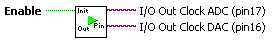
\includegraphics[scale=1]{appendiceA/clock_init}
		\caption{Struttura VI Clock pin init}
	\end{center}
\end{figure}

Questo VI consente di abilitare o disabilitare i pin digitali di uscita che forniscono il clock ai convertitori DAC/ADC della scheda di conversione SCO Board.
\paragraph*{Input}
\begin{itemize}
	\item \textbf{Enable}: Consente di scegliere se abilitare o disabilitare le uscite digitali a cui sono collegati i clock dei convertitori DAC/ADC.
\end{itemize}

\paragraph*{Output}
\begin{itemize}
	\item \textit{I/O out clock ADC}: Indica il pin digitale associato al segnale di clock dell'ADC.
	\item \textit{I/O out clock DAC}: Indica il pin digitale associato al segnale di clock del DAC.
\end{itemize}

\subsection*{Clock generator}

\begin{figure}[H]
	\begin{center}
		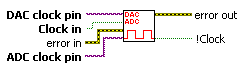
\includegraphics[scale=1]{appendiceA/clock_gen}
		\caption{Struttura VI Clock generator}
	\end{center}
\end{figure}

Questo VI si occupa di generare sulle uscite digitali, relative ai segnali di clock DAC/ADC, il valore logico all'ingresso del VI. Questo VI viene utilizzato per generare il segnale clock per i due convertitori in modo sincrono.

\paragraph*{Input}
\begin{itemize}
	\item \textbf{DAC clock pin}: Indica il pin digitale associato al segnale di clock del DAC.
	\item \textbf{ADC clock pin}: Indica il pin digitale associato al segnale di clock dell'ADC.
	\item \textbf{Clock in}: Valore logico da generare in uscita.
	\item \textit{Error in}: Consente la gestione manuale dell'errore. Questo ingresso viene utilizzato per propagare un codice di errore avvenuto in precedenza nei nodi a monte o per ragioni di sincronizzazione.
\end{itemize}

\paragraph*{Output}
\begin{itemize}
	\item \textit{Error out}: Segnala se l'operazione è avvenuta con successo. In caso di errore viene mostrato un codice di errore.
	\item \textit{!Clock}: Negazione del valore logico in ingresso a \textbf{Clock in}.
\end{itemize}

\subsection*{Single point acquisition}

\begin{figure}[H]  
	\begin{center}
		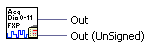
\includegraphics[scale=1]{appendiceA/acquisition}
		\caption{Struttura VI Single point acquisition}
	\end{center}
\end{figure}

Questo VI acquisisce un singolo campione di 12-bit in uscita dall'ADC. In accordo con le specifiche fornite per l'ADC, l'acquisizione del dato sarà eseguita sul fronte di discesa del clock dell'ADC.
Il VI restituisce un valore numerico puro, espresso in \textit{fixed point} da 12-bit e con parte intera da 12-bit. Sono forniti sia il valore con segno che senza segno.

\paragraph*{Input}
Questo VI non ha input

\paragraph*{Output}
\begin{itemize}
	\item \textit{Out}: Valore numerico in uscita dall'ADC, senza segno ($0 \ \div \ +4095$).
	\item \textit{Out (Unsigned)}: Valore in uscita dall'ADC, con segno ($-2048 \ \div \ +2047$).
\end{itemize}

\subsection*{Single point generation}

\begin{figure}[H]  
	\begin{center}
		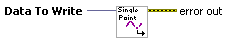
\includegraphics[scale=1]{appendiceA/generation}
		\caption{Struttura VI Single point generation}
	\end{center}
\end{figure}

Questo VI genera un singolo campione da 12-bit sulle uscite della scheda di sviluppo associate agli ingressi del DAC. 
In accordo con le specifiche fornite per il DAC la generazione del dato sarà eseguita sul fronte di salita del clock del DAC. Il VI accetta in ingresso un valore numerico puro, espresso in \textit{fixed point} da 12-bit con parte intera da 12-bit e senza segno (\textit{unsigned}).
\paragraph*{Input}
\begin{itemize}
	\item \textbf{Data to write}: Il dato che si vuole generare in uscita espresso in \textit{unsigned fixed point} ($-2048 \ \div \ +2047$).
\end{itemize}

\paragraph*{Output}
\begin{itemize}
	\item \textit{Error out}: Segnala se l'operazione è avvenuta con successo. In caso di errore viene mostrato un codice di errore.
\end{itemize}

\section*{Esempio di utilizzo del driver}
In questa sezione sarà mostrata la corretta procedura per utilizzare il driver SCO Board all'interno di un progetto LabVIEW.

Il progetto del software LabVIEW che farà uso del driver SCO Board dovrà contenere tutti i VI presenti nell'archivio \textit{.zip} fornito. La struttura delle cartelle contenute nell'archivio non deve essere alterata.

Il progetto avrà la struttura mostrata in figura \ref{progetto}.

\begin{figure}[H]
	\begin{center}
		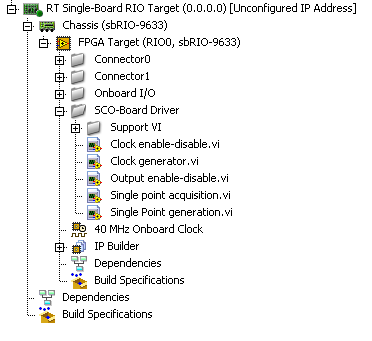
\includegraphics[scale=1]{appendiceA/progetto}
		\caption{Struttura del progetto contenente i driver SCO Board}
		\label{progetto}
	\end{center}
\end{figure}

Invece, il diagramma a blocchi (\textit{Block Diagram}) di un VI che fa uso dei driver SCO Board è mostrato in figura \ref{VI}

\begin{figure}[H]
	\begin{center}
		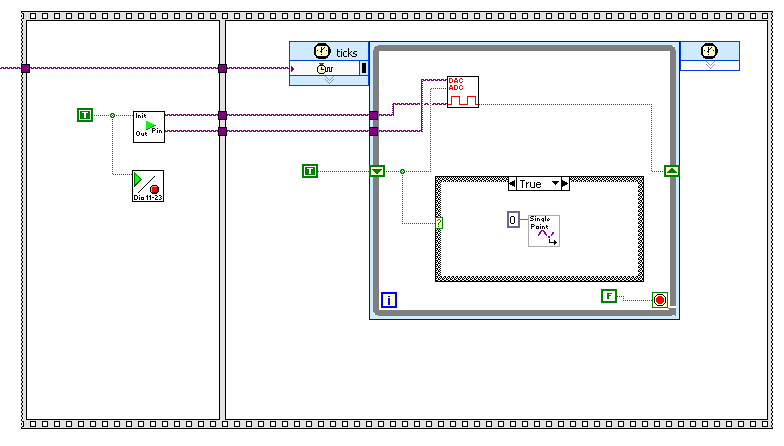
\includegraphics[scale=0.6]{appendiceA/VI}
		\caption{Struttura del VI contenente i driver SCO Board}
		\label{VI}
	\end{center}
\end{figure}

Il VI sarà composto da una \textit{Sequence Structure}: il primo \textit{frame} della struttura avrà il compito di inizializzare le uscite della scheda di sviluppo \textit{sbRIO-9636}, mentre il secondo \textit{frame} conterrà il codice dell'applicazione.

All'interno del codice dell'applicazione è necessario inserire un \textit{Single-Cycle Timed Loop} (SCTL), con frequenza di esecuzione (\textit{Source}) doppia rispetto alla frequenza di campionamento desiderata, che conterrà il VI di generazione del clock (\textit{Clock generator}) e i VI di acquisizione e generazione del segnale (\textit{Single point acquisition} e \textit{Single point generation}). L'utilizzo del SCTL è necessario per garantire una temporizzazione precisa e coerente del clock. La massima frequenza di esecuzione impostabile su SCTL è $100MHz$. Questo, perché i circuiti di conversione della SCO Board possiedono una frequenza massima di campionamento pari a $50MHz$.

All'interno del SCTL sarà inserita, inoltre, una \textit{Case Structure} che garantirà la corretta sequenza e temporizzazione di acquisizione e generazione del segnale. 

In particolare la generazione del segnale sarà eseguita nella scheda \textit{True} della \textit{Case structure} (fronte di salita del segnale di clock), mentre l'acquisizione sarà svolta nella scheda \textit{False} (fronte di discesa del segnale di clock).

Per lo scambio di dati con il resto dell'applicativo è consigliabile utilizzare code FIFO con il pattern \textit{Producer-Consumer}.




